\documentclass[12pt]{article}

\usepackage[a4 paper, top=1in, left=1in,right=1in, bottom=1in,
footskip=0.5in]{geometry}

\usepackage[english]{babel}
\usepackage[utf8]{inputenc}
\usepackage{times}
\usepackage[compact]{titlesec}
\usepackage{graphicx}
\usepackage{enumitem}
\usepackage{colortbl}
\usepackage{float}
\usepackage{acronym}
\usepackage{tocloft}
\usepackage{setspace}
\usepackage{url}
\usepackage[hidelinks,linktoc=all]{hyperref}
\usepackage[backend=biber,style=ieee]{biblatex}

\urlstyle{same}

\titlespacing*{\section}{0pt}{0pt}{0pt}

\onehalfspacing

\definecolor{sea}{RGB}{175,255,215}

\DeclareUnicodeCharacter{0301}{\'\i}

\addto\captionsenglish{
  \renewcommand{\contentsname}
    {Table of Contents}
}

\setlength{\parindent}{0em}
\setlength{\parskip}{1.5pt}

% \titleformat{\section}{\bfseries}{\thesection }{0.5pt}{}
% \titleformat{\subsection}{\bfseries}{}{0.5pt}{}

% \titlespacing*{\section}{0pt}{0pt}{1.5pt}

\graphicspath{{../.img/}}
\addbibresource{references.bib}

\begin{document}

% cover page
\begin{titlepage}

\newcommand{\HRule}{\rule{\linewidth}{0.1mm}}

\begin{center}

  {\huge Purbanchal University}\\[1cm]

  \textbf{\huge College of Biomedical Engineering and Applied Sciences}\\[1cm]


  
\includegraphics[width=0.4\textwidth]{cbeas-logo.png}\\[1cm]

  \color{red} \HRule \\[0.4cm] \color{black}

  {\huge \bfseries Seed-based Functional Connectivity Analysis of
  Hippocampal Network of Patients Suffering from \linebreak Major
  Depressive Disorder}\\[0.2cm]

  \color{red} \HRule \\[2cm] \color{black}

  % Author
  \textbf{\Large \textit{ Proposed By: } \\[5mm]
  \Large
  Lucky Chaudhary [A27] \\
  Namrata Tamang [B3] \\
  Nikin Baidar [B4] \\
  Nilima Sangachchhe [B5] \\
  Shashwot Khadka [B18] \\
  Sneha Khadka [B22] \\ [1mm]
  Suhana Chand [B23]} \\ [1cm]

  \vfill
  {\Large \today}

\end{center}

\end{titlepage}

% preface
\pagenumbering{roman}
\clearpage
\setcounter{page}{1}
\hskip180pt {\textbf{\centering \large Preface} }
\vskip2pt
\addcontentsline{toc}{section}{Preface}

The basis for this project stemmed from the fact that not many
researches have been conducted in Nepal regarding the diagnosis of
mental disorders. Nonetheless, in other countries, many researches and
studies have been conducted regarding the functional connectivity of
different brain regions in depression and other mental
disorders. However, till date, there is no solid evidence that could
be used for the clinical diagnosis of mental disorders. Our project
intends to review past researches and keep up with the studies related
to Major Depressive Disorder and brain functional connectivity. In
addition to that, we have selected hippocampal circuity as the region
of interest for our purposes and the overall project is going to
revolve around how functional connectivity of hippocampal network in
MDD patients differ from that of healthy people.

The following proposal begins with the basic concepts of the resting
state functional connectivity of brain, different regions of brain and
MR images. The concept of MR image processing, functional connectivity
analysis will be used in the project. Making use of these concepts,
our project approaches to compare and come up with a conclusion about
how functional connectivity differs in MDD patients and how the
findings of the project could play a role in diagnosis of MDD. In this
project, the use of ``functional connectivity'' is restricted to mean
quantification of the operational interactions of multiple spatially
distinct brain regions that are not engaged in any specific task or
stimulus. We will further restrict our discussion to connectivity
measures of the hippocampal network, derived from fMRI imaging
modality alone.  We are required to conduct this project as a part of
the curriculum of Biomedical engineering. We hope to acquire
a profound knowledge about MR image processing which would help us
a lot in our career as biomedical engineers. \\ [1cm]

\hspace*{138mm}\textbf{\textit {$-$ Authors}}
\newpage

%abstract
\hskip180pt {\textbf{\centering \large Abstract} }
\vskip2pt
  \addcontentsline{toc}{section}{Abstract}

The absence of biological markers makes it exceptionally difficult for
neurologists to diagnose a person with a mental disorder. Currently,
diagnosis of mental disorders is based on behavioral observations and
patient-reported symptoms, both of which do not have a molecular or an
imaging basis. Although there have been thousands of studies revolving
around the implementation of various imaging modalities for
deciphering the etiology and the physical cause of several mental
disorders, the findings from these studies do not appear amongst the
diagnostic criteria. Meaning that the findings from these studies are
not used for diagnosis purposes. A critical barrier to the clinical
translation of many such findings is the reverse inference fallacy, as
neurological disorders are multifaceted and are influenced by more
than one factor and neuroimaging results can be heavily influenced by
external factors such as patient movement and instrumental
artifacts. However, neuroimaging for diagnosis of mental disorders
seems promising in the future and as a matter of fact, a small
minority of health care providers have already started to implement
neuroimaging techniques such as fMRI, SPECT, PET for the diagnosis of
psychiatric disorders. Nevertheless, there is no solid molecular or
imaging basis that is widely accepted for the assessment of mental
disorders. Here in the proposed research we plan to evaluate
functional network connectivity of the hippocampus in patients with
Major Depressive Disorder based on the MR images of their brain and
investigate the changes in the brain network compared to that of
healthy controls matched according to age and gender.
\newpage

\thispagestyle{empty}
\addcontentsline{toc}{section}{List of Figures}
\listoffigures

\thispagestyle{empty}
\addcontentsline{toc}{section}{List of Tables}
\listoftables
\newpage

% Abbreviations

\begin{center}
  \section*{Abbreviations}
  \addcontentsline{toc}{section}{Abbreviations}
\end{center}

\begin{acronym}

  \acro{ACC}{Anterior Cingulate Cortex}
  \acro{AFNI}{Analysis of Functional Neuroimages}
  \acro{ASN}{Anterior Salience network}
  \acro{BDI}{Beck Depression Inventory}
  \acro{BOLD}{Blood Oxygen Level Dependent}
  \acro{CA}{Cornu Ammonis}
  \acro{DG}{Dentate Gyrus}
  \acro{DMN}{Default Mode Network}
  \acro{DSM}{Diagnostic and Statistical Manual of Mental Disorders}
  \acro{EC}{Entorhinal Cortex}
  \acro{ECN}{Executive Control Network}
  \acro{EEG}{Electroencephalography}
  \acro{fMRI}{Functional Magnetic Resonance Imaging HC Healthy Controls}
  \acro{HPA}{Hypothalamic Pituitary Adrenal}
  \acro{ICA}{Independent Components Analysis}
  \acro{ICD}{International Classification for Diseases}
  \acro{MDD}{Major Depressive Disorder}
  \acro{MFC}{Medial Frontal Cortex}
  \acro{MFG}{Middle Frontal Gyrus}
  \acro{MR}{Magnetic Resonance}
  \acro{OFC}{Orbitofrontal Cortex}
  \acro{PET}{Positron Emission Tomography}
  \acro{PMC}{Premotor Cortex}
  \acro{rFPDD}{Recurrent Familial Pure Depressive Disorder}
  \acro{ROI}{Region of Interest}
  \acro{rs}{Resting State}
  \acro{rsFC}{Resting-state Functional Connectivity}
  \acro{SCA}{Seed-based Correlation Analysis}
  \acro{SPECT}{Single-Photon Emission Computed Tomography}
  \acro{sMRI}{Structural Magnetic Resonance Imaging}
  \acro{SNRI}{Serotonin and Norepinephrine Reuptake Inhibitors}
  \acro{SSRIs}{Selective Serotonin Reuptake Inhibitors}
  \acro{vPFC}{Ventrolateral Prefrontal Cortex}

\end{acronym}

\newpage
% table of contents
\vskip -10pt
\enlargethispage{\baselineskip}
\thispagestyle{empty}
\addcontentsline{}{}{}
\tableofcontents
\newpage

\pagenumbering{arabic}
\clearpage
\setcounter{page}{1}

\section{Introduction}

\subsection{Major Depressive Disorder}

Major Depressive Disorder, generally abbreviated as MDD, is one of the
most common and serious mental disorders. MDD is also referred to as
clinical depression, or just depression as well. MDD can be
characterized by an array of distinct symptoms, some of them being
persistent feelings of sadness, feelings of low self-worth and guilt,
and overall reduced ability to take pleasure from activities that
previously were enjoyable and so on. Although, the exact symptoms of
depression may vary from person to person depending on their
upbringing and various socio-demographic variables such as age, sex,
religious affiliations, employment, income etc. For an individual to
be classified as ``suffering from MDD'', five out of ten symptoms, one
from a set of two and four additional symptoms from another set of
five, must be present during a span of two weeks
\cite{whodepression}. In addition to the symptoms that may be
prevalent in a person suffering from depression, there can be
morphological differences in several brain regions including the
frontal and temporal lobes. On top of that, individuals suffering from
MDD also have abnormal functional connectivity. According to the World
Health Organization, more than 264 million people of all ages suffer
from depression worldwide \cite{whodepression}. Fortunately, there are
effective psychological and pharmacological treatments for moderate to
severe depression. The pharmacological treatment includes medications
such as the SSRIs and SNRI which are two most commonly prescribed
antidepressants. The psychological treatments include psychotherapy
and electroconvulsive therapy, depending on the severity of the
depression.

\subsection{Neuroimaging}

Neuroimaging or brain imaging is the use of various imaging modalities
to either directly or indirectly image the structure, function, or
pharmacology of the nervous system. Current neuroimaging techniques
reveal both form and function. They reveal the brain’s anatomy,
including the integrity of brain structures and their
interconnections. Diagnostic neuroimaging has two prospects, one is
short-term prospects and the other is long-term prospects. The
near-term or short-term prospects of diagnostic neuroimaging allows
validation of the categories of neuro-disorders rather than in the
criteria for diagnosing an individual patient. On the other hand,
long term prospects allow diagnostic distinctions that are difficult
to make on the basis of behavioral observations alone, so potentially
distinctive patterns of brain activation identified through imaging
will be useful. Neuroimaging can be divided into two broad categories:

\begin{enumerate}

  \item \textbf{Structural Imaging}, which deals with the structure of
    the nervous system and the diagnosis of gross (large scale)
    intracranial disease (such as a tumor) and head injury.

  \item \textbf{Functional imaging}, which is used to diagnose
    metabolic diseases and lesions on a finer scale (such as
    Alzheimer’s disease) and also for neurological and cognitive
    psychology research and building brain-computer interfaces
    \cite{neuroimaging}.

\end{enumerate}

Functional Magnetic resonance imaging (fMRI) is a modern technique of
imaging, which is a powerful non-invasive and safe tool used for the
study of the function of the brain based on the measure of the brain
neural activation. The fMRI can localize the location of activity in
the brain which is caused due to sensory stimulation or cognitive
function. In the clinical setting, fMRI allows the researchers to
study how healthy brain functions, how different diseases affect the
brain functions, how brain functions altered due to disease or injury
can be restored, and how drugs can control the disease’s effect on
brain activity \cite{fMRI}.

\subsection{Brain Networks}

A brain network, on a large scale, can be defined as a collection of
brain regions working together to produce a specific function. Brain
networks can be identified at different resolutions, therefore there
is no universal atlas of brain networks that fits all
circumstances. However, based on converging evidence from related
studies, there are six large-scale, core brain networks that are most
widely accepted due to their stability
\cite{estimatingLargeScaleNetworks}. The following figure is
a diagrammatic representation of the core brain networks:

\begin{figure}[H]
  \centering
  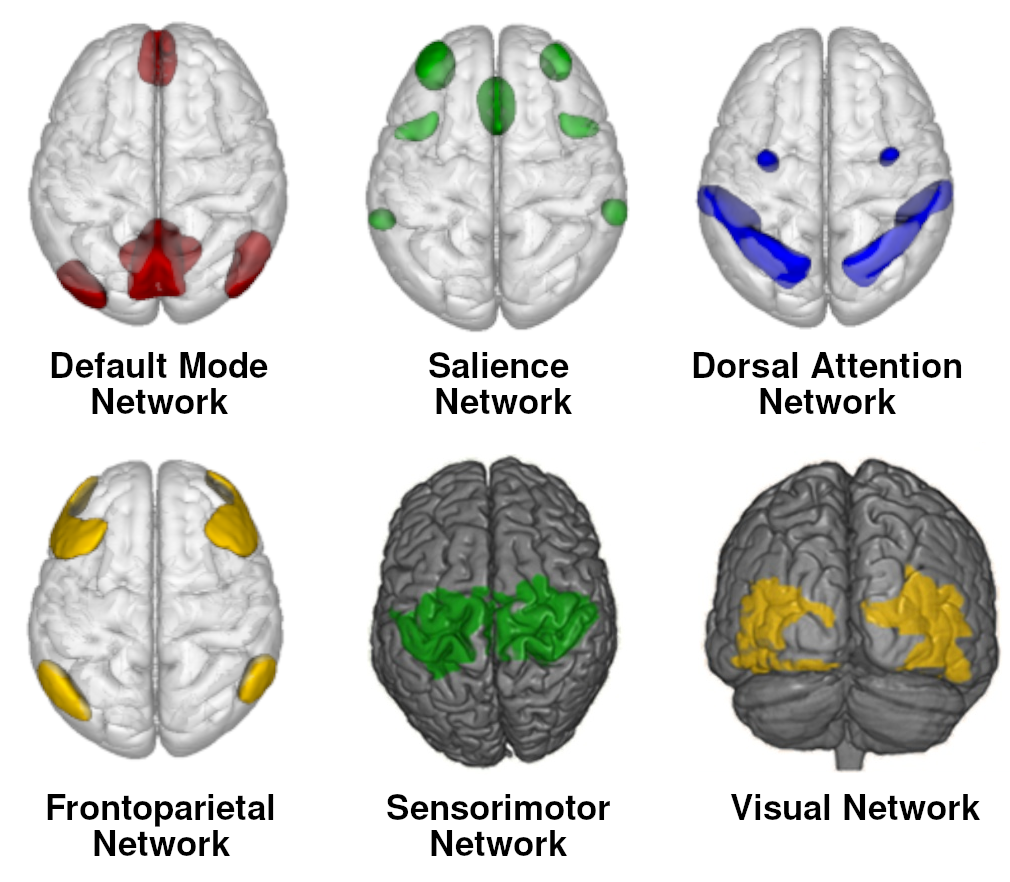
\includegraphics[width=0.8\textwidth]{brain-networks.png}
  \caption{Core Brain Networks}
  \cite{dorsalattentionfronto}\cite{Majorbrainnetworks}
\end{figure}

\newpage

\begin{enumerate}

  \item \textbf{Default Mode Network:} This network is active when an
    individual is awake and at rest \cite{serendipitousDMN}.

  \item \textbf{Salience Network:} Monitors the salience of external
    inputs and internal brain networks
    \cite{saliencemetabolic}\cite{functionalconnectivity}.

  \item \textbf{Dorsal Attention Network:} Involved in voluntary,
    top-down deployment of attention \cite{thomasorganization}.

  \item \textbf{Frontoparietal Attention Network:} Initiates and
    modulates cognitive control \cite{frontoparietalAttentionFunc}.

  \item \textbf{Sensorimotor Network:} Processes somatosensory
    information and coordinates motion \cite{heine2012resting}.

  \item \textbf{Visual Network:} This network handles visual
    information processing \cite{brainvisual}.

\end{enumerate}

There are more subsets of these six networks such as the limbic,
auditory, right/left executive, cerebellar, spatial attention,
language, lateral visual, temporal and visual perception/imagery. An
emerging paradigm in neuroscience is that cognitive tasks are
performed not by individual brain regions working in isolation but
rather by brain networks consisting of several discrete brain regions
that are said to be ``functionally connected''. The functional
connectivity of brain networks can be acknowledged through
(statistical) analysis of images acquired through a variety of
techniques such as the fMRI, EEG, PET or SPECT
\cite{wikibrainnetworks}.

\subsection{Resting State Functional Connectivity}

Functional connectivity can be defined as the temporal correlation
between spatially remote neurophysiological events, expressed as
deviation from statistical independence across these events in
distributed neuronal groups and areas. In simple terms, functional
connectivity refers to the communication be tween functionally
distinct brain regions \cite{functionalConnectivityNikin}. The results
of the study conducted by Bharat B. Biswal et. al. suggests that while
variations in blood flow might contribute to functional connectivity
maps, BOLD signals play a dominant role in the mechanism that gives
rise to functional connectivity in the human brain
\cite{biswalsimultaneous}. During resting conditions, our brain
remains functionally and metabolically active. The fact that brain
remains ``metabolically active'' means there will be consumption of
oxygen which results in fluctuations in the BOLD signal. Spontaneous
fluctuations in distinct brain regions show temporal correlations with
each other, reveling complex patterns of functional connectivity
\cite{biswal1995functional}.

\begin{figure}[H]
  \centering
  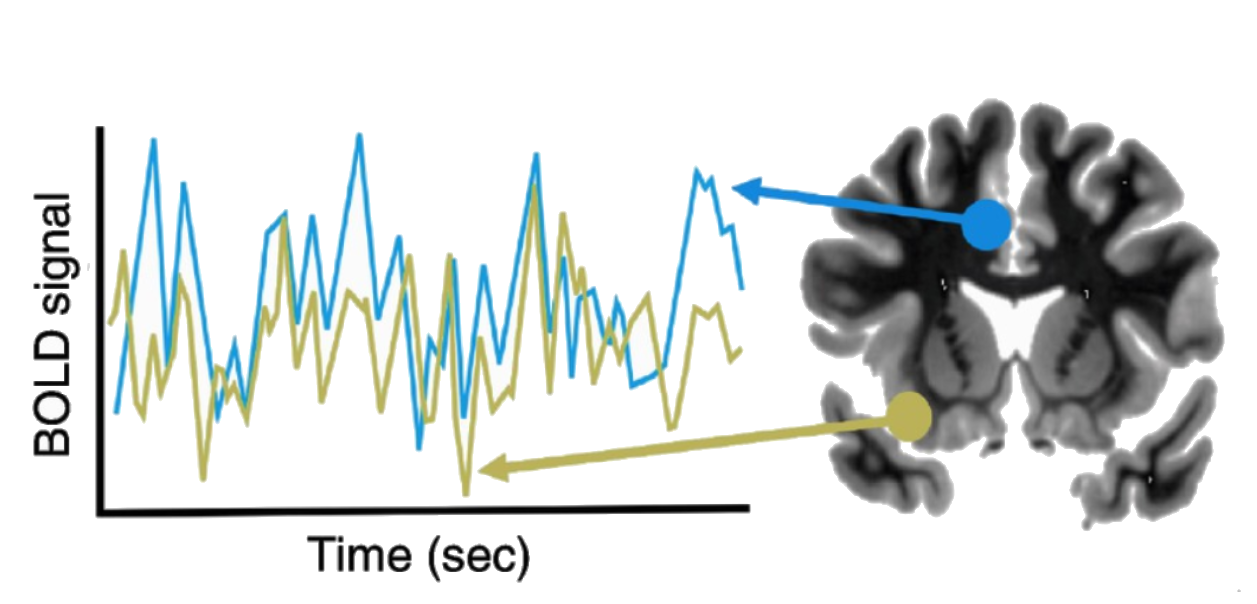
\includegraphics[width=0.8\textwidth]{rsfc.png}
  \caption{Schematic Representation of Bold Signal Fluctuations}
\end{figure}

In the above diagram, the solid blue line represents the BOLD signal
of one brain network and the green line represents that of
another brain network. Now, the resting state functional connectivity
can be defined as the correlation patterns in the spontaneous
fluctuations in BOLD signal in the absence of any stimulus or task
\cite{frontiers:rsfc}. Resting-state functional connectivity measures
the temporal correlation of spontaneous Blood Oxygen Level Dependent
(BOLD) signals among spatially distributed brain regions, with the
assumption that regions with correlated activity form functional
networks. There are two methods that are most commonly used to examine
resting state functional connectivity of brain networks, they are as
follows:

\begin{enumerate}[nosep]
  \item Seed-based Correlation Analysis (SCA) and
  \item Independent Components Analysis (ICA)
\end{enumerate}

In seed-based approaches, activity is extracted from a specific region
of interest and correlated with the rest of the brain. In contrast,
ICA does not begin with pre-defined brain regions. It is
a multivariate, data driven approach that deconstructs fMRI
time-series data throughout the brain into separate spatially
independent components \cite{connectivityanalysis}. The resting-state
fMRI study produces reliable and reproducible results, and several
features of resting-state fMRI makes it favorable for investigating
the functional correlation of various brain regions in psychiatric and
neurological disorders. First, compared to the modular representations
of traditional fMRI, functional connectivity provides a broader
network representation of the functional architecture of the
brain. Second, the absence of an explicit task eases the cognitive
demand of the fMRI environment, thereby eliminating the problem of
whether or not to match groups on task performance and allowing
researchers to investigate under-studied populations, including
infants and cognitively impaired individuals. Finally, the relatively
standard manner in which resting-state fMRI data are acquired makes it
ideal for multi-site investigations and data sharing \cite{resting}.

\newpage

\section{Objectives}

The objectives of the project are as follows:

\subsection{General Objectives}

\begin{itemize}

  \item Perform analysis of the functional connectivity of the
    hippocampus in patients suffering from Major Depressive Disorder
    and acquire a comprehensive idea about how it compares to that of
    normal individuals of the same age group and sex.

\end{itemize}

\subsection{Specific Objectives}

\begin{itemize}

  \item Deploy computational tools, and implement image processing
    algorithms for the exploration of MR image datasets of the human
    brain using AFNI.

  \item Explore data visualization tools, with emphasis on displaying
    functional brain networks.

  \item To perform Seed-based Analysis  to explore functional
    connectivity within the brain based on the time series of a seed
    voxel or Region of Interest (ROI).

\end{itemize}


\newpage

\section{Problem Statement} % \vskip -16pt

\subsection{Need For An Imaging Basis} % \vskip -16pt

Current diagnostic procedures involved in diagnosis of mental
disorders do not have an imaging or a biochemical basis
\cite{nobiochemicalbasis} \cite{noimagingbasis}. The diagnosis
procedures that are the gold standard for the diagnosis of psychiatric
disorders are wholly based on behavioral observations and patient
reported symptoms. Two most widely established symptoms are used to
classify these manifestations, one is the Diagnostic and Statistical
Manual of Mental Disorders (DSM) and the other is International
Classification for Diseases (ICD). Despite each being, widely used as
the other, both of these diagnosis manuals are more like frameworks
that provide a way of classifying a psychiatric disorder depending on
patterns of behaviour rather than interpreting the etiology and the
physical cause of those disorders. This statement alone raises an
argument that ``although reliable, current diagnostic procedures in
psychiatry are not entirely valid''.

Let us take an example of the diagnostic procedure involved in the
diagnosis of Major Depressive Disorder. The DSM-V, published in 2013,
is the most up-to-date manual and is based upon the work of expert
study groups and makes use of large sets of data. According to the
DSM-V, for a person to be classified as ``suffering from Major
Depressive Disorder'', he/she must report with either depressed mood
or anhedonia (inability to feel pleasure in normally pleasurable
activities) along with four out of eight additional symptoms
\cite{diagnosticbrainimaging}. This makes it possible for two distinct
individuals who do not share a single symptom in common and to receive
similar treatment (or medication) for MDD. Furthermore, the current
diagnostic procedures such as the DSM-V are not perfect. For example,
impulsivity, emotional lability (the property of changing rapidly),
and difficulty with concentration each occur in more than one
disorder. Now, the fact that different exemplars of the same category
can share no symptoms and that the exemplars of two different
categories may share common symptoms, raises questions about the
validity of the current diagnostic procedures in psychiatry. In
addition to that, some other medical conditions such as thyroid
disease, brain tumors, and vitamin deficiency can mimic
depression-like symptoms \cite{externalfactorsinMDD}. Therefore,
a diagnosis may also have to be conducted in order to rule out some
other medical condition that might be causing depressive symptoms. For
instance, a blood test can be done to ensure the symptoms are not due
to thyroid related issues.

\subsection{Reverse Inference Fallacy}

In the present day and world, a variety of imaging modalities such as
ultrasonography, x-rays, computed tomography, MRI, SPECT, PET,
fluoroscopy, etc are being implemented for a large number of purposes,
most of them include clinical diagnosis of various diseases and the
others include research. Now, while some of these imaging modalities
such as MRI, SPECT and PET are indeed being used for research that
involves the diagnosis of psychiatric disorders, they are yet to be
implemented for the actual diagnosis of mental disorders. There exist
thousands of published research studies using functional neuroimaging
methods such as SPECT, PET, and fMRI that revolve around diagnosis of
mental disorders. In spite of that, the findings from these research
do not appear amongst the diagnostic criteria; aside from its use to
identify potential physical injury or tumours, neuroimaging is not
used in diagnostic procedure in psychiatry.

The fact that advanced imaging techniques are not being used for
diagnosis of mental disorders, especially after so many researchers
have done studies on this regard, may seem a bit counter-intuitive at
first but the arguments produced by reverse inference against it is
quite sensible and valid. Reverse inference is a kind of reasoning
that is applied to infer the involvement of a specific cognitive
process from observed brain activation during a task. It attempts to
uncover specific cognitive processes or behaviours that my be
associated with specific structural or functional brain alterations.

However, reasoning backwards from brain activity is problematic
because neurological disorders, such as MDD, are multifaceted and are
influenced by several factors such as concurrent diseases, disease
history and artifacts. For example, in the following figure we can see
that a radiologist can assure that a person’s arm is broken or not by
taking a look at the radiograph. However, a radiologist cannot assure
a patient is suffering from this particular mental disorder my taking
a look at the CT scan of the patient’s brain due to reverse inference
fallacy.

\begin{figure}[H]
  \centering
  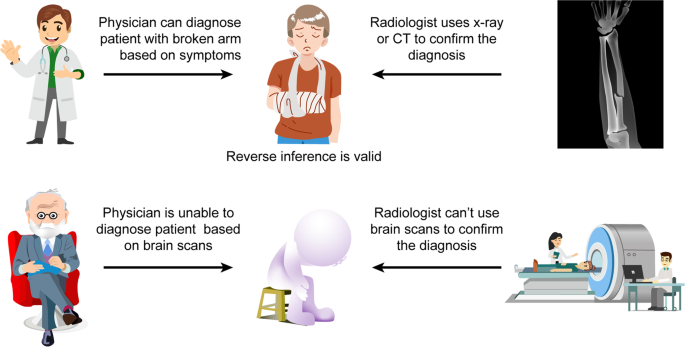
\includegraphics[width=\textwidth]{reverse-inference.png}
  \caption{Illustration of reverse inference fallacy in diagnostic
  psychiatry}
\end{figure}

Most psychiatric imaging studies involve subjects from only two
categories: patients from a single diagnostic category and people
without any psychiatric diagnosis (healthy individuals), the most that
can be learned from such a study is how brain activation in those with
a particular disorder differs from brain activation in those without
a disorder. This raises a dilemma for the diagnosing clinician, as the
question is not ``does this person have disorder X or are they
healthy?'' but rather ``does this patient have disorder X,Y,Z or are
they healthy?'' because the pattern of images that distinguishes
patients with disorder X from healthy people may not be unique to
X but shared with a other disorders.

In addition to the reverse inference fallacy, standardization is
another issue that contributes to neuroimaging not yet finding
a place in psychiatric practice. Standardization is relevant in the
sense that protocols for imaging studies differ from study to study,
particularly amongst functional imaging studies. Findings on the
patterns of activation acquired in studies of psychiatric patients
depend strongly on the task being performed by the subjects and the
statistical comparisons made by the researcher afterwards. Such
findings are pretty much incomplete unless they include the
information about which task evoked the activation in question:
whether the patient wa resting, processing emotional stimuli,
resisting emotional stimuli or engaged in some other task? Therefore,
the fact that the imaging study’s conclusions are relative to the
tasks performed adds further complexity to the problem of consistently
discriminating patterns of activation of healthy and ill subjects.

Now, in the word of technology that is advancing day in day out,
development of more sophisticated methods of image analysis may hold
promise discerning the underlying differences among the many disorders
that feature similar regional abnormalities. Nevertheless, the scope
of neuroimaging seems promising for the aid in the diagnosis, and
hopefully treatment of psychiatric disorders. Considering the above
mentioned arguments, an imaging basis for the diagnosis of mental
disorders seems like the need of the hour.

\newpage
\section{Review of Literature}

\subsection{Background}

Efforts are continuously being made to discover reliable biomarkers
for the clarification of biological mechanisms that are involved in
psychiatric disorders, identification of subjects at risk and provide
etiology-based treatments. Imaging modalities such as structural
magnetic resonance imaging (sMRI) and functional magnetic resonance
imaging (fMRI) are used to outline brain irregularities over Major
depressive disorder (MDD)\cite{structuralbrainimaging}
\cite{fMRIFuture}. Multiple imaging modalities have been considered
for the assessment of functional connectivity of brain networks, but
fMRI is the most commonly used amongst the others. This is mostly
because fMRI imaging methods such as echo-planar sequences are
sensitive to changes in the blood oxygenation level dependent (BOLD)
signal that reflects neuronal activation \cite{rogersassessing}. Most
studies that have been referred to, whilst writing this review have
utilized the fMR-imaging modality to conduct investigations on the
core aspects of functional brain alterations in patients suffering
from MDD. The goal of this literature review is to gain comprehensive
knowledge about the associations of various brain networks with Major
Depressive Disorder and also to acquire a brief overview of how the
brain networks, especially the hippocampal network, gets affected by
MDD. Since this project is mostly concerned with the hippocampal
network, most of the literature will more or less be related to the
temporal lobe and its structures.

\subsection{Functional Magnetic Resonance Imaging for the Assessment
of MDD}

People with MDD show distinct structural and functional alterations
that differ from those of healthy individuals. Unlike structural brain
imaging that captures the anatomical structures present in the brain,
functional brain imaging involves measurement of blood flow and
metabolism to visualize the activation of specific brain
regions. Nearly all fMRI studies utilize blood oxygenation
level-dependent (BOLD) fMRI for assessing functional brain
activity. A brain region becomes active when there is blood flow in
that region, and an elevated level of metabolism. Brain activation
results in increased consumption of oxygen, which increases the inflow
of oxygenated blood and leads to an elevated BOLD signal. BOLD fMRI
allows for regional and global mapping of brain regions activated
during non-task (i.e. rest) and task-related activities
\cite{zhuo2019rise}. fMRI comes in two flavours, one is the
resting-state fMRI and the other is the task-based fMRI. ``Resting
state'' is when a person is fully awake but isn’t performing any
particular stimulus or task that requires attention and
cognition. While many studies are based on the rs-fMRI, researchers
believe that the rs-fMRI lacks the linearity and stationary signals
required for the assessment of MDD.

\newpage
Several researches and evidence have found reduced hippocampal volumes
in depressed patients compared with healthy controls. Videbech and
Ravnkilde discovered that hippocampal volumes were 8–10\% smaller in
patients with MDD when compared with healthy controls
\cite{zhuo2019rise}. Likewise, Bremner et al. found that left
hippocampal volumes were ~19\% smaller in MDD patients when compared
with healthy controls\cite{zhuo2019rise}. \textcite{zhuo2019rise}, in
their paper have also showed functional alterations in the activity of
the right hippocampus, right para-hippocampal gyrus, left amygdala and
the entire caudate nucleus, which ultimately suggests that the
temporal lobe and various structures in the temporal lobe, such as the
hippocampus might have important pathophysiology of MDD. Therefore,
additional studies are needed to determine the relevance of these
findings.

In a task based fMRI study, Fu et. al. found that presentation of sad
faces led to increased activation of the left hippocampus, mainly the
amygdala and the parahippocampal gyrus \cite{correlation}. It shows
the evidence that MDD patients have a hard time recognizing and
processing emotion in facial expression (sad vs. happy).

\subsection{Resting State Functional Connectivity of Hippocampal
Networks}

There has been a plethora of studies that focus on the abnormal
functional connectivity of several brain networks in patients with
MDD. A lot of these studies show that MDD not only shows associations
with regional deficits, but also with abnormal functional integration
of distributed brain regions. Several brain regions with abnormal
activities in the resting-state have been identified to be associated
with MDD, such as the para-hippocampal gyrus, prefrontal cortex,
cingulate gyrus, fusiform gyrus, and thalamus. Moreover, disruptions
in functional connectivity have been observed between specific pairs
of regions in MDD through functional connectivity analyses which may
or may not include seed-based correlation analysis \cite{homogeneity}.

\textcite{frontiers:rsfc} used the independent component approach
(ICA), selecting a set of regions with shared fMRI signal fluctuations
and a high degree of spatial similarity to the DMN, and reported
increased connectivity with the thalamus and the subgenual ACC in
depression. Many studies have found that the hippocampus, which is
a complex structure embedded deep into the temporal lobe, plays an
important role in MDD. Hippocampus can be subdivided into
3 sub-structures, and these structures are listed below:

\begin{enumerate}[nosep]
  \item  Cornu Ammonis (CA)
  \item  Dentate Gyrus (DG)
  \item  Subiculum
\end{enumerate}

Various studies have been performed with each of these sub-structures
as the seed or the region of interest. \textcite{rightinsula} found
increased connectivity in the left premotor cortex (PMC) and reduced
connectivity in the right insula with the CA seed region. Similarly,
increased connectivity was reported in the left orbitofrontal cortex
(OFC) and left ventrolateral prefrontal cortex (vPFC) with the DG seed
region. The subiculum seed region revealed increased connectivity with
the left premotor cortex (PMC), the right middle frontal gyrus (MFG),
the left ventrolateral prefrontal cortex (vPFC) and reduced
connectivity with the right insula. In addition to that,
region-of-interest based correlation analyses performed on rs-fMRI
data showed positive functional connectivity between the hippocampus
in limbic system, subcortical areas, temporal lobe, medial and
inferior prefrontal cortex, while at the same time, negative
functional connectivity was in bilateral prefrontal cortex, parietal
and occipital cortex and the cerebellum
\cite{cerebellum}. Furthermore, multiple research has implicated
abnormalities in the prefrontal-hippocampal neural circuitry in
patients suffering from MDD \cite{prefrontal}. fMRI studies have also
found abnormal hippocampal activation as well as abnormal functional
connectivity of prefrontal-hippocampus circuitry in adults who were
suffering from MDD. Moreover, Peng et. al. in one of their recent
studies reported decreased rsFC between hippocampus and insula in
medication-resistant adult patients \cite{pengetal}.

The hippocampus has been proven to play an important role in memory
\cite{memory} and emotion processing \cite{emotion}. Functional
abnormalities of the hippocampus in adult MDD have been consistently
reported in several fMRI studies. According to an fMRI study,
decreased brain activity in the hippocampus was reported in depressive
patients. The hippocampus and the amygdala of MDD patients showed an
overlapping pattern of reduced FC to the dorsomedial-prefrontal cortex
and fronto-insular operculum. Both of these regions are known to
regulate the interactions among intrinsic networks (i.e., default
mode, central executive, and salience networks) that are disrupted in
MDD \cite{disruptedMDD}. A few postmortem studies have found decreased
cellular density in the hippocampus, including one study that showed
patients with MDD have fewer anterior dentate gyrus granule cells than
control subjects \cite{controlsubject}. However, functional imaging
studies at this resolution in patients with MDD are lacking.

\enlargethispage{\baselineskip}
For several reasons, researchers have focused on the role of the
hippocampus in depression. The hippocampus is involved in the
regulation of the hypothalamic pituitary adrenal (HPA)-axis, which is
responsible for the production of stress-related glucocorticoids such
as cortisol \cite{cortisol}. In this context, depressed individuals
have been found consistently to report high levels of stress
\cite{stress}, which is reflected biologically in elevated rates of
hypercortisolemia and disturbed HPA-axis functioning. Moreover,
depressed patients have also been found to be characterized by
difficulties in hippocampal-dependent learning and memory
\cite{learning}. Also, Problems can occur when excessive amounts of
cortisol are sent to the brain due to a stressful event or a chemical
imbalance in the body.

\newpage
\subsection{Overview of Hippocampal Circuitry and its Functions}

Hippocampus is a complex brain structure embedded deep into temporal
lobe. It has a major role in learning and memory. Hippocampus can can
be related to the functional requirement of episodic memory and more
specifically to the storage and retrieval of memory
\cite{hippocampal}. The hippocampus is part of the hippocampal
formation which includes the DG (Dentate Gyrus), the hippocampus
proper, and the subiculum gyrus \cite{limbic}. The hippocampal gyrus
contains areas such as the EC (entorhinal cortex) and subiculum, which
are both vital in the flow of information through the hippocampus. The
following figure\cite{hippocampalcircuitry} is a schematic
representation of the hippocampal circuitry:

\begin{figure}[H]
  \centering
  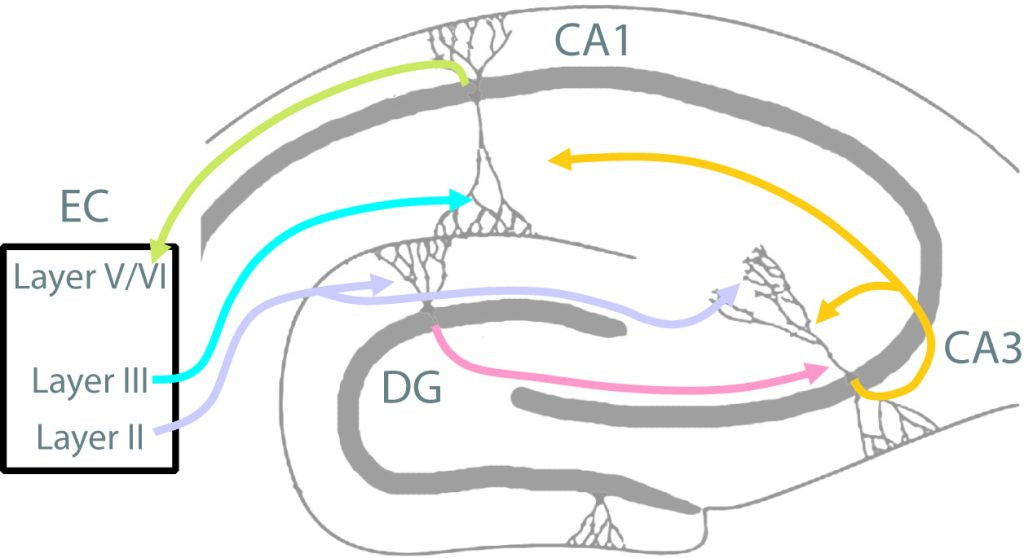
\includegraphics[width=0.75\textwidth]{hippocampal-circuitry.jpg}
  \caption{Schematic Representation of Hippocampal Circuitry
  }
\end{figure}

The neural circuit in the hippocampus is referred to as the
hippocampal circuitry, or as the trisynaptic. The hippocampal circuit
is divided into CA1, CA2, CA3, CA4, EC and the DG regions. These
regions coordinate information from a variety of sources. Some inputs
to the hippocampus arrive from the entorhinal cortex pass through to
the DG. From the DG, connections are made to CA3 of the hippocampus
via mossy fibers and then to CA1 via Schaffer collaterals. From these
two CA fields information then passes through the subiculum entering
the alveus, fimbira and fornix and then to other areas of the brain.

Information flows into and through the hippocampus via. three
principal pathways \cite{limbicsystem:hippocampus}:

\begin{enumerate}
  \item The perforant pathway: From the entorhinal cortex to granule
    cells of the DG.

  \item The mossy fiber pathway: From the granule cell of the dentate
    gyrus to the pyramidal cells of the CA3 region of the hippocampus.

  \item The Schaffer collateral pathway: From the CA3 region to the
    CA1 region of the hippocampus.

\end{enumerate}

The CA1 region has an important role in memory due to the high levels
of NMDA glutamatergic receptors located in the CA1 Schaffer collateral
neurons. The synaptic plasticity of these neurons heavily relies on
long-term potentiation (LTP) induction to allow the strengthening of
declarative memory which includes two types of implicit memory:
episodic and semantic memory such as facts and events. CA2 is a small
region located between CA1 and CA3. It is often ignored due to its
small size. The CA3 is a portion of the hippocampal formation adjacent
to the dentate gyrus. \textcite{hippocampalca3} have found that the
CA3 plays an essential role in the consolidation of memories when
examining CA3 regions using the Morris water maze.

The entorhinal cortex (EC) is a structure in the brain located in the
medial temporal lobe. The EC is composed of six distinct layers. The
superficial (outer) layers, which includes layers I through III, are
mainly input layers that receive signals from other parts of the
EC. The deep (inner) layers, layers IV to VI, are output layers, and
send signals to different parts of the EC and the brain. Layers II and
III project to the CA3 area of the hippocampal formation (via the
perforant path) and to the granule cells of the dentate gyrus,
respectively. The dentate gyrus (DG) is the innermost section of the
hippocampal formation. The dentate gyrus consists of three layers:
molecular, granular, and polymorphic.The granule cells (present in
granular layer) are the major source of input of the hippocampal
formation, receiving most of their information from layer II of the
entorhinal cortex, via the perforant pathway. Information from the DG
is directed to the pyramidal cells of CA3 through mossy fibres.

\subsection{Important FCs for Diagnosis of MDD}

Default mode network (DMN), Anterior salience network (ASN) and
Executive control network (ECN) are the brain networks linked with
clinical depression. Increased functional connectivity within the DMN
is primarily associated with depression. At the same time, it is found
that the DMN-ECN and the DMN ASN pairs have fewer interactions or
connectivity during episodes of depression. Within the ECN, the
functional connectivity may be excessive or deficient. Furthermore,
the ECN in depressed women is correlated with negative self-directed
thoughts and the ECN-DMN functional connectivity is related to
rumination. Researches have shown that ASN which includes main
emotional areas maybe over, under or normally connected in
depression. Depression is also related with the impaired functional
connectivity of other brain networks besides the ones mentioned
above. In addition to that, the Posterior Cingulate Cortex, which is
a part of the DMN has shown significant relationship with the
hippocampal network, albeit this is not just specific to MDD.

\textcite{LRbrainnetwork}, on comparing the functional activity within
DMN, found that there was decreased functional connectivity within DMN
network in depressed people, which contradicted most research that
have been conducted. This may be because the patients involved in
their study had mild to moderate depression which showed similar
cognitive features as in depression (MDD) like rumination and control
deficits, but lacked neural markers present in typical serious
condition like MDD. Many studies that have been published showed
increased functional connectivity within DMN in depression, which was
found to be contradiction with one particular research which may be
due to sample differences like severity of the disorder, age group,
and other demographics.

Significant rs-fMRI differences between groups were identified in
multiple clusters in the DMN and ECN. Greater positive connectivity
within the ECN and between ECN and DMN regions was associated with
poorer episodic memory performance in the group of healthy individuals
but better performance in the MDD group. Greater connectivity within
the DMN was associated with better episodic and working memory
performance in the Non-Depressed group but worse performance in the
MDD group. These results provide evidence that cognitive performance
in MDD may be associated with aberrant functional connectivity in
cognitive brain networks and suggest patterns of alternate brain
function that may support cognitive processes in MDD. Results also
showed that the DMN–left fronto-parietal network is the pair
discriminating between healthy and depressed people to the highest
degree. According to Davidson and Heller models, left prefrontal
activity is related to positive emotions and motivations, while right
corresponds to negative emotions and withdrawal of motivation
\cite{model}. Relatively active right prefrontal area and idling left
prefrontal cortex together may be a neurophysiological signature of
depression. Therefore, coupling of left prefrontal with DMN denotes
its passivity and that there is less approach motivation, less happy
mood which is one of the most important depression related
signs. Increased functional connectivity between left fronto-parietal
network and subsystems of the DMN can be seen in fMR images of
depressed patient.

\subsection{Structural Changes associated with MDD}

The latest research \cite{brainvolume} shows that the size of specific
brain regions can decrease in people who experience
depression. Researchers continue to debate which regions of the brain
can shrink due to depression and by how much. Hippocampus, thalamus,
amygdala and the frontal and prefrontal cortices are the regions that
have reported the most shrinkage. The amount by which these areas
shrink is linked to the severity and the length of the depressive
episodes. In the hippocampus, for example, noticeable changes can
occur anywhere from 8 months to a year. \cite{effectMDD}

\textcite{brainshrink}, in her newspaper article stated that people
experiencing their first depressive episode had a normal hippocampus
size but as the number of episodes of depression a person had would
increase, the greater the reduction in hippocampus size. It has been
widely reported that there is a significant reduction in hippocampal
volume in depression patients. This situation was found in both adult
and adolescent depressed patients, whether they were in their first or
recurrent depressive episodes. A recent study reported that, in female
patients with recurrent familial pure depressive disorder (rFPDD),
volumetric reductions of the right hippocampal body and tail were
significantly larger than those of the left, while the whole brain
volume was approximately equal to that of healthy subjects. There is
evidence that stress via the hypothalamic pituitary-adrenal axis can
result in elevated glucocorticoid levels in patients with depression
and can act on the glucocorticoid receptors in the hippocampus. Thus,
hippocampal atrophy occurs as a result. Reduced gray matter volume and
reduced functional activity in the hippocampus would lead to negative
emotion and the inability of cognitive processing in depressive
patients. Depression can also decrease neuronal dendrite branching and
plasticity in the hippocampus.

In addition, depression can trigger activation of the
hypothalamic-pituitary-adrenal axis, increase the level of
corticosteroids, and down regulate hippocampal
neurogenesis. Depression makes changes in hippocampal volumetric
changes, hippocampal neurogenesis, and apoptosis of hippocampal
neurons \cite{effectMDD3}.

\subsection{Reverse Inference Fallacy in MDD}

\vspace{-5pt}
The diagnosis of MDD relies heavily on patients for symptom
recall. Like in many other mental disorders there is no specific
physical symptom in MDD, therefore neurologists are unable to deduce
MDD based on conventional MRI. Moreover, different mental disorders
can produce similar structural or functional brain alterations which
puts the neurologist in a much greater dilemma as they are unable to
determine whether a specific alteration in the brain is attributed to
MDD-alone. So, the reverse inference is invalid as structural or
functional activity patterns from MRI cannot be used to diagnose
a patient with a specific neurological disorder. Researchers, over the
past few decades have been attempting to develop a ``bridge'', such as
novel biomaterial, high resolution and multi-modality imaging
technique, artificial intelligence, novel nanomaterials and
quantitative electrical signal acquisition technologies to overcome
the reverse inference fallacy that hinders the study of
MDD. \cite{zhuo2019rise}

\subsection*{Conclusion of the Literature Review}

Evidence shows that major depressive disorder (MDD) patients at
resting-state brain connectivities are aberrant compared with healthy
controls (HC). Abnormal resting-state functional connectivities of
distributed brain networks are believed to contribute to the MDD
illness process. Reliable, reproducible and valid conclusions must be
derived from these types of studies, for imaging modalities such as
fMRI to not only aid in the diagnosis but also to optimize patient
care, reduce treatment resistance and shorten the duration of illness.

\vspace{-5pt}
\enlargethispage{\baselineskip}
After a thorough review of the literature, fMRI looks promising for
providing excellent and reliable indexes for the aid in the diagnosis
and ultimately treatment of MDD. Once it overcomes the aforementioned
hurdles, fMRI imaging technique could become a clinical decision
support tool that might reduce unsuccessful treatments and improve
treatment efficacy and efficiency of mental disorders all together.

\newpage
\section{Feasibility Study}

The following points addresses the feasibility of the proposed study:

\begin{itemize}

  \item This project will primarily focus on analysis of the
    functional connectivity of the hippocampal network of patients
    suffering from Major Depressive Disorder.

  \item  Although the approach of neurological study is new in Nepal,
    thousands of research has been conducted worldwide that involves
    similar approaches for the exploration of functional connectivity.

  \item Publicly available dataset will be used in this project. The
    MR images of MDD patients as well as that of healthy individuals
    for this project are retrieved form the DecNef Project Brain Data
    Repository. Data used in the preparation of this work were
    obtained from DecNef Project Brain Data Repository gathered by
    a consortium as part of the Japanese Strategic Research Program
    for the Promotion of Brain Science (SRPBS) supported by the
    Japanese Advanced Research and Development Programs for Medical
    Innovation (AMED). \textcite{dataset}

  \item There are not many materials or components required for the
    project. We will be using open-source softwares such as Analysis
    of Functional Neuro Images (AFNI) and the Linux operating system,
    this adds to the feasibility of this project.

  \item Furthermore, all the work involved in this project can pretty
    much be conducted virtually at home, therefore this eliminates the
    obstacles that may arise due to the on-going pandemic.

  \item Hence, the feasibility study to conduct this proposed project
    is positive and supportive.

\end{itemize}
\newpage

\section{Methodology}

\subsection{Methods and Materials}

Functional Magnetic Resonance Imaging is well established as a method
for the detection and delineation of regions of the brain that change
their level of activation in response to specific conditions. fMRI
studies, such as the one we will be conducting, implement imaging
methods that are sensitive to fluctuations in the BOLD (Blood Oxygen
Level Dependent) signal that reflects neuronal activation.  Therefore,
our methodology will approach the study of functional connectivity
using BOLD signals, and since we will will perform seed-based
analysis, these BOLD signals will be restricted to only a specific
region of interest. We will adopt seed-based resting stat fMRI
connectivity analysis in order to study alternations in functional
connectivity of hippocampus region of fifteen volunteers suffering
from major depressive disorder and compare the results with that of
fifteen well-matched healthy controls. In addition to that, we will
also attempt to explore how the changes in functional connectivity of
MDD patients affect their emotional behaviour and memory.

We will use AFNI (Analysis of Functional NeuroImages). AFNI is one of
the leading software suite of C, Python and R programs and shell
scripts primarily developed for processing, analyzing and
visualization of three dimensional human brain functional magnetic
resonance imaging results. AFNI has a rich software package for
processing and displaying fMRI data. In addition to that, several
statistical analysis methods for 3D functional datasets are also
available in this software. AFNI is an open-source software that was
developed for reasearch purposes, however it is not cross-platform and
only runs on UNIX based operating systems such as MacOS and Linux
based systems like Ubuntu, Fedora, Linux mint, CentOS and Arch
Linux. We will be running AFNI on Linux based systems.

\subsection{Seed Based Functional Connectivity Analysis}

Seed-based functional connectivity, also referred to as Region of
Interest-based functional connectivity, finds regions that correlate
with the activity in the seed region. In seed-based analysis, the
correlation is compared between the time-series of the seed or the ROI
and the rest of the brain. The correlation between different brain
regions indicate that they are involved in the same underlying
functional process and thus are interpreted as functionally
connected. ``Functionally connected'' does not necessarily mean that
these brain regions are directly connected by neuronal fibers. The
overall connectivity of the brain will be visualized using AFNI. The
main advantage of seed-based analysis is that the computation is
simple and the interpretation of the results is intuitive. But as the
seed region changes, the results of the functional connectivity will
also change which is this method's demerit.

\subsection{Region of Interest Selection}

For our study, we have chosen the hippocampus as the seed region or
the region of interest. The reason for which we have chosen the
hippocampus as our region of interest is three folds, one, since we
are using publicly available dataset we had to settle for a suitable
data that the repository had. Two, although there have been many
studies about the functional connectivity other brain regions, there
have been limited reports of functional alterations in the temporal
lobe with the use of rs-fMRI imaging modality. The third reason for
which we have chosen hippocampus to be our reason of interest is, MDD
being associated with alterations in regional brain volumes,
particularly hippocampus along with the functional changes in brain
circuits makes it more convenient to ponder upon the hippocampal
region of brain as the ROI. Therefore, our study will be centered
towards the hippocampal region of the limbic system.

\subsection{fMRI Data Acquisition}

As mentioned earlier, we will be using the \textcite{dataset} public
repository to acquire the fMRI images of patients diagnosed with major
depressive disorder, as well as those of healthy controls. The brain
imaging dataset that we plan to use for this project initially will
have 3T MRI images of 1410 participants that were collected at 11
different sites. However, we will only be using a tiny fraction of
this big data. Statistical approaches will be undertaken (statistical
tests will be performed) in order to narrow down this big data to just
30 subjects.

\enlargethispage{\baselineskip} The \textit{SRPBS Multidisorder MRI
Dataset} public repository has categorized the data set into two
groups, healthy controls (HC) and depressed patients (MDD). There are
more than 1410 subjects in this repository out of which only fifteen
right handed volunteers from each category, the MDD patients and the
HC, will be chosen. For the volunteers form the depressed category,
only subjects whose BDI was greater than 30 will be selected. Since we
will be acquiring the data from large scale public dataset, diagnosed
by neurologist, this assures our research to be tilted more to
accuracy and efficiency. All the participants, extracted from the
public data set, have underwent a standardized clinical evaluation
protocol, which included a general and neurological examination, which
will make our research more feasible. Once selection of volunteers is
complete, we will proceed to match both groups according to their age
and sex. Since sex is a categorical variable, chi square test will be
performed to measure the appropriateness of fit. For matching the age,
t-test will be used to calculate the p-value.

The authenticity of the data acquired from the above mentioned dataset
is guaranteed as the participants from the depressed category had
undergone a standardized clinical evaluation protocol, which included
a general as well as a neurological examination performed by licensed
neurologists.

\newpage
\subsection{Image Pre-processing}

Image pre-processing is the most important aspect of our
project. Pre-processing is an important step which converts the raw
fMRI data into a form that is understandable by each software package.
Pre-processing is also important to improve the signal quality of the
raw data obtained from the MRI scanner. Image pre-processing will
involve steps like artifact detection, baseline correction,
realignment, movement correction, co-registration, normalization, and
smoothing.

The fMRI data will be preprocessed using AFNI \cite{coxafni}. Various
different toolboxes will be used for fMRI preprocessing which will
involve spatial or temporal filtering of the fMRI data and improving
the image resolution. In addition to these steps, motion correction
will also be done in order to minimize of the noise produced in the
image due to artifacts. Seed based resting-state functional
connectivity (rsFC) analysis of hippocampal network will be performed
such that for each seed region, rsFC will be calculated as the
correlation between its mean time course and the time course of every
voxel in the brain. Seed-voxel correlation mapping is one of the
simplest techniques for studying functional connectivity: the
correlation coefficient between the fMRI signal at different times and
measurements of activation in the seed region will be calculated
separately for each voxel in the brain and will be displayed
a parametric image. The final rsFC results, between the MDD patients
and HC will be compared using statistical approach.

\subsection{Statistical Analysis of Functional Connectivity}

\enlargethispage{\baselineskip}
\vspace{-5pt}
Once the rs-fMR images from the public data set has been
pre-processed, statistical tests will be implemented to for a thorough
analysis of the functional connectivity of the seed. Specifically, we
plan to assess functional connectivity between various regions of the
brain and hippocampal area. To assess functional connectivity in the
brain region, Resting-state analyses, that is, time series
correlations in BOLD fMRI data acquired in a task-free state will be
used. A statistical approach to image analysis makes it possible to
discover spatial and temporal patterns that correspond to the
performance of specific tasks and specific diagnoses. Such statistical
methods have only begun to be applied to clinical disorders but show
promise for increasing the ``specificity'' of brain imaging markers
for mental illness.

\newpage

\section{Cost Estimations}

We have chosen AFNI (Analysis of Functional Neuro Images) in order to
conduct this project. AFNI is a software, primarily developed for the
analysis and display of multiple MRI modalities such as fMRI
images. AFNI is an open-source software which runs on UNIX based
operating systems such as macOS or Linux. Due to the high price of
a computer from Apple Inc., we have chosen to run AFNI on top of
a Linux operating system. Since, both AFNI and the Linux operating
systems are free and open-source softwares, the cost of this project
becomes extremely low. In addition to using free softwares, the data
that we plan to use for this project is also available freely from the
\textcite{dataset} public repository which further cuts down the cost
of this project.

Nevertheless, we will require an SSD (Solid State Drive) on top of
which we will install the Linux operating system and an external HDD
for storing the data acquired from the public repository, the external
HDD will allow us to easily carry and move the data amongst each
other. Furthermore, if the findings from our project seems to be
beneficial to the field of diagnostic psychiatry, we expect financial
aid from the university concerning the release of our findings for
academic journals or research papers.

The budget plan for this project is tabulated below:

\begin{table}[H]
  \newcolumntype{P}[1]{>{\centering\arraybackslash}p{#1}}
  \centering
    \begin{tabular}{|c|m{5cm}|c|P{1.5cm}|P{1.5cm}|P{2.5cm}|}
      \hline
      S.N. & \multicolumn{1}{c|}{Cost Element} & Cost Remarks & Rate
      (NRs.) & Quantity (Unit) & Total Cost (NRs.)\\ \hline
      1 & SANDISK SATA SSD (512 GB) & Fixed & 8,500 & 4 & 34,000 \\ \hline
      2 & External HDD (1 TB) & Fixed & 4,000 & 1 & 4,000 \\ \hline
      3 & Miscellaneous & Variable & - & - & 7,000 \\ \hline
      \rowcolor{sea}
      4 & \multicolumn{4}{c|}{Grand Total} &
      \multicolumn{1}{c|}{45,000} \\ \hline
  \end{tabular}
  \caption{Cost Estimations}
\end{table}

So, the total cost estimation \cite{ssdprice} of this project is
\textit{NRs.\hspace*{2pt}45,000 only}.

\newpage

\section{Proposed Work Flow}

The following chart represents our plans regarding how we wish to
proceed in this project.

\begin{figure}[H]
  \centering
  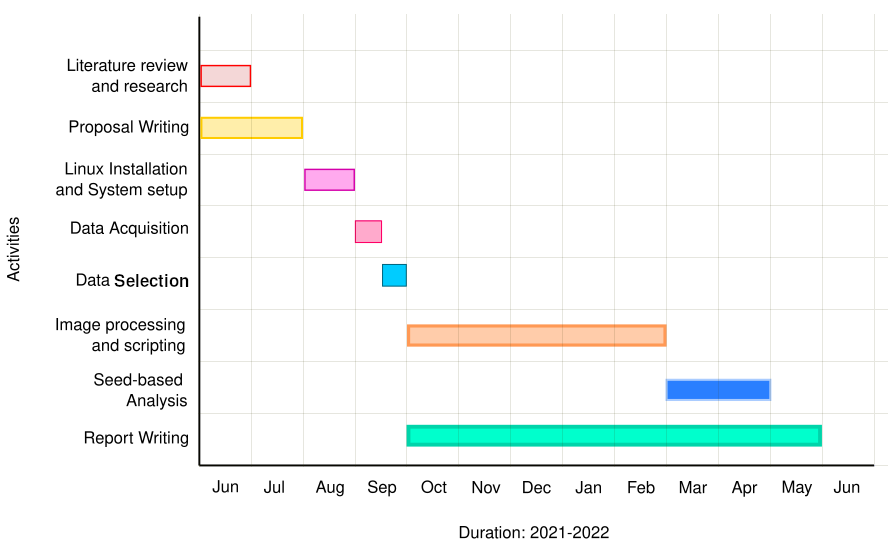
\includegraphics[width=1\textwidth]{proposed-workflow.png}
  \caption{Gantt Chart illustrating the proposed workflow}
\end{figure}

\section{Conclusion}

Previous studies indicated discrepant functional connectivities
between MDD patients and HC. However, it is unknown whether these
connectivities can be used as diagnostic biomarkers of MDD.18 Indeed,
whether the future diagnostic models built on the functional
connectivity values can improve treatment prediction and clinical
outcome depend on its accuracy performance.

While the results might not be sufficient to provide a detailed
understanding of the complex and changing functional connectivity of
the brain which could make actual diagnosis of MDD, this project can
lay the foundations for further research and development.

\newpage

\section*{References}
\addcontentsline{toc}{section}{References}
\printbibliography[heading=none]

\end{document}
